\section{Az EGTIB bemutatása}
\begin{frame}
	\frametitle{Az EGTIB bemutatása}
	\begin{block}{Az EGTIB projekt célja}
		\begin{itemize}
			\item felhasználóbarát felület
			\item lehetőség a daganatos sejtek modellezésére 
			\item szimulációk megjelenítése
			\pause
			\item a szimulációs eredmények megjelenítésére
		\end{itemize}
	\end{block}

	\begin{figure}[ht!]
		\centering
		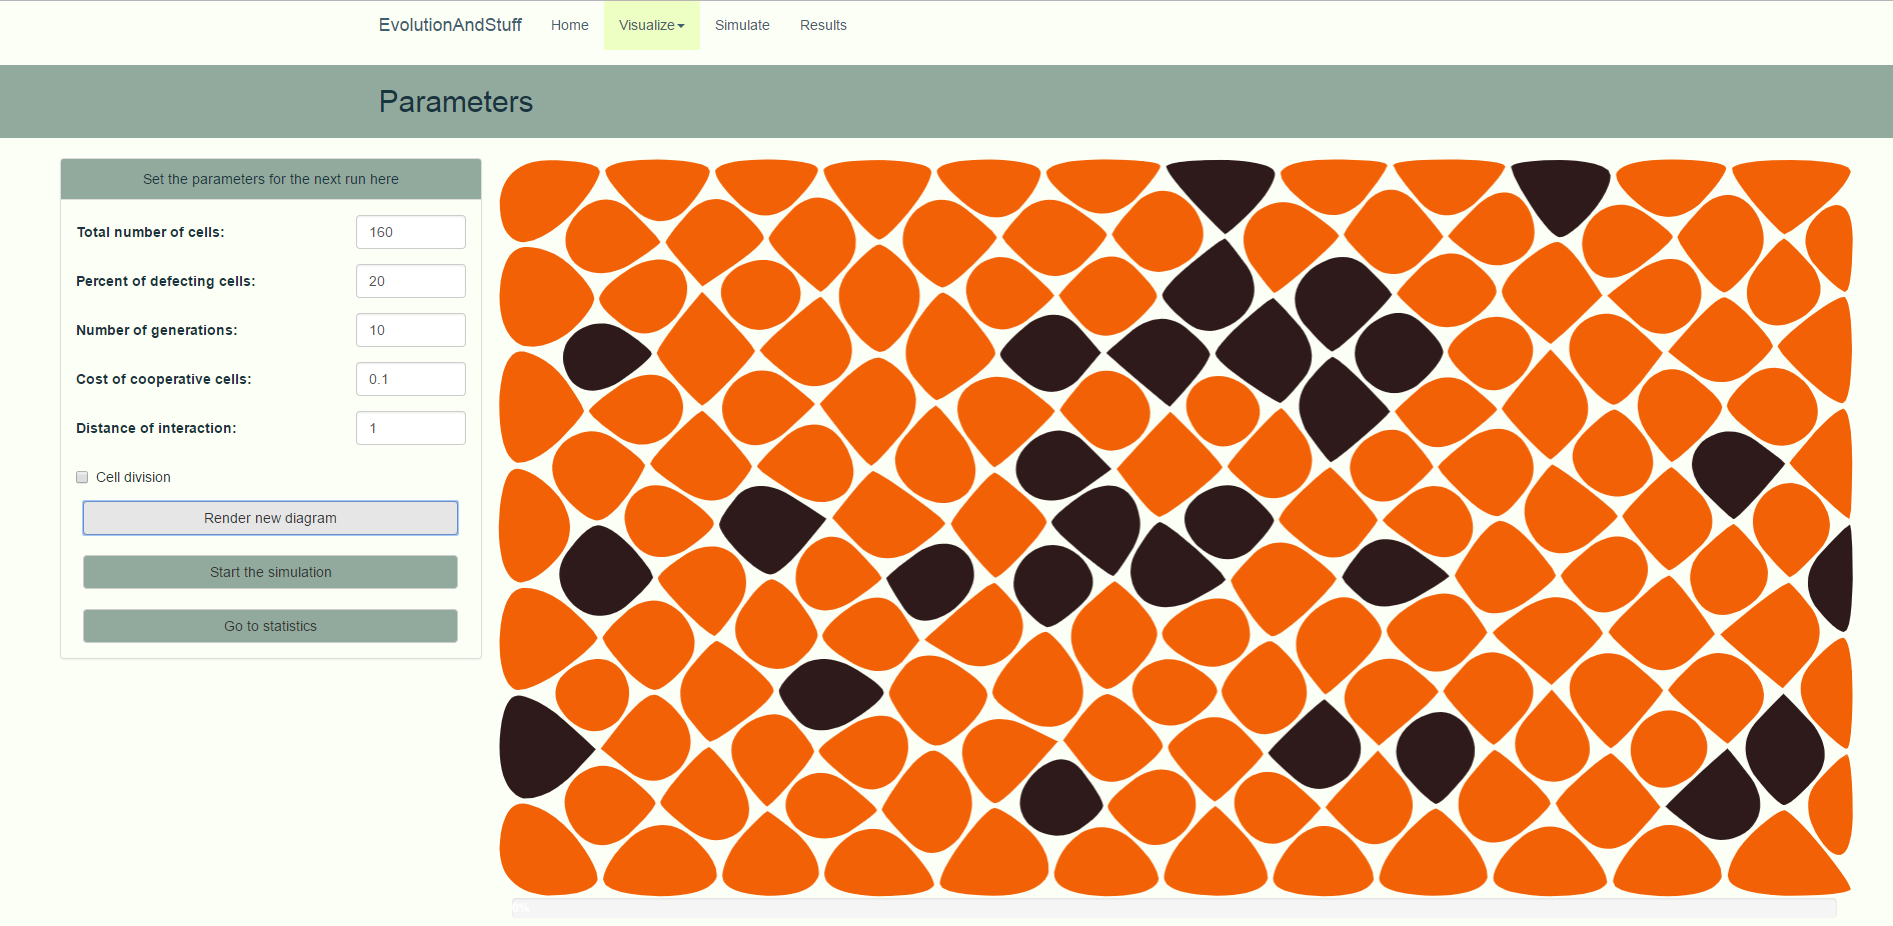
\includegraphics[width=0.6\linewidth]{images/voronoi_page.png}
		\caption{Pillanatkép az alkalmazásról}
		\label{fig:SimulateWithDiagram}
	\end{figure}
\end{frame}

\subsection{Funkcionalitások}
\begin{frame}
	\frametitle{Funkcionalitások}
	\begin{block}{Választható paraméterek}
		\begin{itemize}
			\item kezdeti populáció mérete
			\item defektálók aránya 
			\item generáció szám (szimuláció hossza)
			\item kooperáló sejtek termelési költsége 
			\item diffúziós távolság mérete
			\item legyenek a sejtek osztódásra képesek?
		\end{itemize}
	\end{block}
\end{frame}

\begin{frame}
	\frametitle{További választható paraméterek}
	\begin{block}{}
		\begin{equation}
		V(j) = 1/[1 + e^{(-s(j-k)/n)}]
		\end{equation}
		\begin{itemize}
			\item k - az áthajlási pont helye
			\item s - a függvény meredeksége a áthajlási pontban
			\item n - a csoport mérete
		\end{itemize}
	\end{block}
	\begin{block}{}
		\begin{equation}
		g(i) = 1/[1 + e^{(-z(i-d)/D)}]
		\end{equation}
		\begin{itemize}
			\item z - a függvény meredeksége a áthajlási pontban
			\item d és D - a diffúziós gradiens alakja
		\end{itemize}
	\end{block}
\end{frame}

\begin{frame}
	\frametitle{Demó}
	\Huge{\centerline{Demó}}
\end{frame}